\chapter{等离子体、导体与电介质中的电磁波}\label{ch:b2:waves-in-media}

短波广播依靠在高层大气上反射而横跨大洋，
高层大气像镜子一样将其反射——同一层大气却让
电视和卫星信号穿透过去。金属勺子闪闪发光，
微波炉门上的金属网能把微波挡在里面，同时
你仍可透过它看着食物加热；一块玻璃对光透明，
却对紫外线不透明。在每种情形中，波进入
某种材料，材料中的电荷发生响应，而这种响应改变了
波：它的速率、衰减，甚至它能否
传播。本章讨论介质的三种标准模型——自由电子
气体、欧姆导体和束缚电子——并用唯一的一种方法统一处理：
把感应电流加入
麦克斯韦方程组，然后读出色散关系。

\section{等离子体中的波}

\begin{definition}[等离子体；自由电子模型]\label{def:b2:waves-in-media:plasma}
\index{等离子体}\index{等离子体频率}
\emph{等离子体}是由自由电子（数密度为 $n$，质量为 $m$，电荷为 $-e$）
与正离子组成的、整体呈电中性的气体，其中离子质量为电子的数千倍，
可视为固定不动。高层大气（电离层，
$n \sim 10^{11}$--$10^{12}$ m$^{-3}$）、气体放电管、日冕，
以及——在光频段——金属中的传导电子，
都是等离子体。忽略碰撞（波的周期比
两次碰撞之间的时间短得多）。其特征频率为
\emph{等离子体频率}
\[
\omega_p = \sqrt{\frac{ne^2}{\varepsilon_0m}} , \qquad
f_p = \frac{\omega_p}{2\pi} \approx 9\,\text{赫兹}\times\sqrt{n\,[\text{m}^{-3}]} :
\]
对电离层为 \qty{3}{MHz} 至 \qty{9}{MHz}，对金属为 \qty{2e15}{Hz}
（紫外波段）。
\end{definition}

\begin{theorem}[等离子体的色散关系]\label{thm:b2:waves-in-media:plasmadispersion}
\index{截止频率（等离子体）}\index{倏逝波（等离子体）}
对等离子体中的横向 PPH 波 $\underline{\vect E} = \underline{\vect E}_0\eu^{\iu(\omega t - kx)}$，
电子以 $\underline{\vect v} = -e\underline{\vect E}/\iu m\omega$ 振动，
并携带电流密度 $\underline{\vect j} = \underline\gamma\underline{\vect E}$，其中
$\underline\gamma = ne^2/\iu m\omega$；由麦克斯韦方程组可得
\[
k^2 = \frac{\omega^2 - \omega_p^2}{c^2} .
\]
在 $\omega_p$ 以上，波可以传播，并有 $v_\varphi = c/\sqrt{1 - \omega_p^2/\omega^2}
> c$，$v_g = c\sqrt{1 - \omega_p^2/\omega^2} < c$，$v_\varphi v_g = c^2$；在
$\omega_p$ 以下，$k = -\iu\kappa$，其中 $\kappa = \sqrt{\omega_p^2 - \omega^2}/c$，此时波
为\emph{倏逝波}，穿透深度为 $1/\kappa$，并发生全反射
（见\cref{ch:b2:wave-interfaces}）；等离子体于是起着镜子的作用。当 $\omega
\gg \omega_p$ 时，电子跟不上振荡，等离子体是透明的。
\end{theorem}

\begin{proof}
运动方程为 $m\,\dd\vect v/\dd t = -e\vect E$（磁力
$ev B \sim evE/c$ 在 $v \ll c$ 时可忽略，离子的运动则
小 $m/M$ 倍）：$\iu m\omega\underline{\vect v} = -e\underline{\vect E}$。于是
$\underline{\vect j} = -ne\underline{\vect v}$。对横波，等离子体保持
电中性（$\vect k\cdot\vect E = 0$ 由高斯定律给出 $\rho = 0$），故
麦克斯韦–安培定律为 $-\iu\vect k\wedge\underline{\vect B} = \mu_0\underline\gamma\underline{\vect E}
+ \iu\omega\mu_0\varepsilon_0\underline{\vect E}$，麦克斯韦–法拉第定律为 $\underline{\vect B} = \vect k
\wedge\underline{\vect E}/\omega$；联立得 $k^2\underline{\vect E} = \mu_0(\iu\omega\underline\gamma -
\omega^2\varepsilon_0)(-1)\underline{\vect E}$，即 $k^2 = \omega^2\mu_0\varepsilon_0 - \iu\omega\mu_0
\underline\gamma = (\omega^2 - ne^2/\varepsilon_0m)/c^2$。速度的求法与
\cref{ch:b2:dispersion-wave-packets}中相同。
\end{proof}

\begin{remark}[能量去向]\label{rem:b2:waves-in-media:plasmaenergy}
电导率为纯虚数：$\langle\vect j\cdot\vect E\rangle = 0$，
电子在半个周期内从波中吸取能量，
并在下一个半周期内交还给波——这是一种无耗介质，波的能量
在场与电子的动能之间分配，
并以 $v_g$ 传播。碰撞为 $\underline\gamma$ 添加一个小的实部，
并产生微弱的吸收：电离层的 D 层在白天吸收中波，
这就是远处的调幅电台在夜间能被收到的原因。
\end{remark}

\begin{example}[电离层与无线电]\label{ex:b2:waves-in-media:ionosphere}
在 F 层中 $n = \qty{1e12}{m^{-3}}$，$f_p = \qty{9}{MHz}$。低于此频率的短波
广播被反射（并可在电离层与地面之间来回跳跃，绕地球传播），
调频（\qty{100}{MHz}）、电视
和卫星通信则穿透过去。频率为 \qty{3}{MHz} 的波仅能穿入
$1/\kappa = c/\sqrt{\omega_p^2 - \omega^2} = \qty{6}{m}$ 的深度，然后
折返。重返大气层的航天器被
一层 $n \sim 10^{18}$ m$^{-3}$、$f_p \sim \qty{10}{GHz}$ 的等离子体包裹，
数分钟内失去无线电联系。
\end{example}

\begin{omfigure}
\begin{tikzpicture}
\begin{axis}[omaxis, axis x line=bottom, axis y line=left, width=6.2cm, height=4.6cm,
    xlabel={$kc/\omega_p$}, ylabel={$\omega/\omega_p$}, xmin=0, xmax=3, ymin=0, ymax=3.3, xtick={1,2,3}, ytick={1,2,3}, samples=80,
    xlabel style={at={(axis description cs:0.5,-0.12)}, anchor=north},
    ylabel style={at={(axis description cs:-0.12,0.5)}, rotate=90, anchor=south},
    legend style={font=\scriptsize, at={(0.97,0.05)}, anchor=south east, draw=none, fill=none}]
  \addplot[omThm, thick, domain=0:3] {sqrt(1+x*x)};
  \addplot[omDef, dashed, domain=0:3] {x};
  \addplot[black, dotted] coordinates {(0,1) (3,1)};
  \legend{等离子体, $\omega = ck$}
  \node[font=\scriptsize, anchor=west] at (axis cs:0.1,0.5) {倏逝};
\end{axis}
\end{tikzpicture}
\hfill
\begin{tikzpicture}[font=\small, x=1cm, y=1cm, >=Stealth]
  \draw[thick] (-3.4,0) -- (3.4,0); \node[font=\footnotesize] at (2.9,-0.3) {地面};
  \draw[omExo, thick, dashed] (-3.4,2.6) -- (3.4,2.6); \node[omExo, font=\footnotesize] at (2.6,2.85) {电离层，$n_e$};
  \draw[omThm, thick, ->] (-3.0,0) -- (-1.5,2.55); \draw[omThm, thick, ->] (-1.5,2.55) -- (0,0.0); \draw[omThm, thick, ->] (0,0) -- (1.5,2.55); \draw[omThm, thick, ->] (1.5,2.55) -- (3.0,0);
  \node[omThm, font=\footnotesize] at (-2.2,1.6) {$f < f_p$};
  \draw[omDef, thick, ->] (-1.0,0) -- (0.4,3.3) node[right, font=\footnotesize] {$f > f_p$};
\end{tikzpicture}

{\small 左：等离子体的色散关系——在
$\omega_p$ 以下无传播，以上为趋近光线的双曲线。右：
等离子体频率以下的短波被电离层反射，
在地球周围往复跳跃；更高频率则逸入太空。}
\end{omfigure}

\section{欧姆导体中的波：趋肤效应}

\begin{theorem}[趋肤效应]\label{thm:b2:waves-in-media:skin}
\index{趋肤效应}\index{趋肤深度}
在欧姆导体中（$\vect j = \gamma\vect E$，$\gamma$ 为实数，频率
满足 $\omega\tau \ll 1$ 及 $\varepsilon_0\omega \ll \gamma$，即对铜而言低于 $\sim\qty{1e16}{Hz}$
）时，位移电流可忽略，场满足
扩散方程 $\Delta\vect E = \mu_0\gamma\,\partial_t\vect E$。一列 PPH 波
在 $x = 0$ 处进入导体后满足
\[
\underline k^2 = -\iu\mu_0\gamma\omega , \qquad \underline k = \frac{1 - \iu}\delta , \qquad
\delta = \sqrt{\frac2{\mu_0\gamma\omega}} ,
\]
于是 $\underline E = E_0\,\eu^{-x/\delta}\eu^{\iu(\omega t - x/\delta)}$：它
在\emph{趋肤深度} $\delta$ 内衰减，相位也
每经过 $\delta$ 相位转过一弧度——波长 $2\pi\delta$，相速度 $\omega\delta \ll
c$。电流 $\vect j = \gamma\vect E$ 集中在表面以下
厚度为 $\delta$ 的薄层内，$\vect B$ 滞后 $\vect E$ \qty{45}{\degree}，且
$|B| = |E|\sqrt2/\omega\delta$。对铜，在 \qty{50}{Hz} 时 $\delta = \qty{9.2}{mm}$，
在 \qty{100}{kHz} 时为 \qty{0.21}{mm}，在 \qty{1}{GHz} 时为 \qty{2.1}{\micro m}。
\end{theorem}

\begin{proof}
$\operatorname{\vect{curl}}\vect B = \mu_0\gamma\vect E$（略去位移电流），并且
$\operatorname{\vect{curl}}\vect E = -\partial_t\vect B$，对后者取旋度：
$-\Delta\vect E = -\mu_0\gamma\partial_t\vect E$（导体呈电中性，$\operatorname{div}
\vect E = 0$）。对 $\eu^{\iu(\omega t - kx)}$，有 $k^2 = -\iu\mu_0\gamma\omega$，且
$\sqrt{-\iu} = (1 - \iu)/\sqrt2$，得 $\underline k = (1 - \iu)/\delta$（取
在导体内衰减的那个根）。由法拉第定律，$\underline B = \underline k\underline E/\omega = (1 - \iu)
\underline E/\omega\delta$，模为 $\sqrt2E/\omega\delta$，相位为 $-\pi/4$。
\end{proof}

\begin{omfigure}
\begin{tikzpicture}
\begin{axis}[omaxis, axis x line=middle, axis y line=left, width=7.0cm, height=4.4cm,
    xlabel={$x/\delta$}, ylabel={$E/E_0$}, xmin=0, xmax=6, ymin=-1.1, ymax=1.15, xtick={0,2,4,6}, ytick={-1,1}, samples=200,
    xlabel style={at={(axis description cs:1.0,0.5)}, anchor=west},
    ylabel style={at={(axis description cs:-0.08,0.5)}, rotate=90, anchor=south}]
  \addplot[omThm, thick, domain=0:6] {exp(-x)*cos(deg(x))};
  \addplot[omDef, dashed, domain=0:6] {exp(-x)};
  \addplot[omDef, dashed, domain=0:6] {-exp(-x)};
\end{axis}
\end{tikzpicture}
\hfill
\begin{tikzpicture}
\begin{axis}[omaxis, axis x line=bottom, axis y line=left, width=6.4cm, height=4.4cm,
    xmode=log, ymode=log, xmin=10, xmax=1e10, ymin=1e-7, ymax=1e-1,
    xlabel={$f$ (Hz)}, ylabel={$\delta$ (m)}, xtick={1e1,1e3,1e5,1e7,1e9}, ytick={1e-6,1e-4,1e-2},
    xlabel style={at={(axis description cs:0.5,-0.12)}, anchor=north},
    ylabel style={at={(axis description cs:-0.14,0.5)}, rotate=90, anchor=south}, samples=50,
    legend style={font=\scriptsize, at={(0.97,0.95)}, anchor=north east, draw=none, fill=none}]
  \addplot[omThm, thick, domain=10:1e10] {sqrt(2/(4*pi*1e-7*6e7*2*pi*x))};
  \addplot[omDef, thick, domain=10:1e10] {sqrt(2/(4*pi*1e-7*5*2*pi*x))};
  \legend{铜、海水}
\end{axis}
\end{tikzpicture}

{\small 左：导体内部的场——一个衰减振荡，
在数个趋肤深度内即衰减殆尽。右：铜与海水的趋肤深度
随频率的变化：工频下为毫米量级，
吉赫下为微米量级；海水只让最长的无线电波穿透。}
\end{omfigure}

\begin{example}[趋肤效应的应用]\label{ex:b2:waves-in-media:skinuses}
\index{交流电阻}\index{法拉第笼}
（i）半径 $a \gg \delta$ 的导线，电流集中在一个
厚度为 $\delta$ 的环带中：其电阻由 $1/\gamma\pi a^2$ 增至约 $1/\gamma
2\pi a\delta$ 每米——对一根 \qty{1}{mm} 的铜线，
在 \qty{1}{MHz} 时为直流值的四倍，在 \qty{1}{GHz} 时为一百倍。高频线圈
常用“利兹线”（多股相互绝缘的细线）或镀银管；电网
导线则为绞合线，外包铝护套。（ii）
金属盒使波衰减为 $\eu^{-d/\delta}$ 倍（$d$ 为所穿过的厚度）：
厚 \qty{1}{mm} 的铝外壳能将 \qty{1}{MHz} 衰减 \qty{100}{dB}，而对 \qty{50}{Hz}
几乎不起作用——低频磁场需要铁来屏蔽。（iii）
潜艇只能接收甚长波无线电（$\delta = \qty{2.3}{m}$ 对应
\qty{10}{kHz}，在海水中）；水雷则借线圈在其中感生的
涡流而被探测（见\cref{ch:b2:maxwell-equations}，扩散
时间为 $\mu_0\gamma d^2$）。
\end{example}

\section{电介质中的波：束缚电子}

\begin{proposition}[弹性束缚电子；复折射率]\label{prop:b2:waves-in-media:lorentz}
\index{电介质}\index{极化强度}\index{极化率}\index{复折射率}\index{洛伦兹模型}
在绝缘体中，每个电子都束缚于其原子：偏离平衡的位移
$\vect r$ 会引起回复力 $-m\omega_0^2\vect r$，并
伴有阻尼 $-m\Gamma\,\dd\vect r/\dd t$（能量被辐射或传给
晶格）。在波的驱动下，$m\ddot{\vect r} = -m\omega_0^2\vect r - m\Gamma\dot{\vect r}
- e\vect E$；位移的电子使介质具有\emph{极化强度}
（单位体积的偶极矩）$\vect P = -ne\vect r = \varepsilon_0\underline\chi(\omega)
\underline{\vect E}$，\emph{极化率}为
\[
\underline\chi(\omega) = \frac{\omega_p^2}{\omega_0^2 - \omega^2 + \iu\Gamma\omega} ,
\qquad \omega_p^2 = \frac{ne^2}{\varepsilon_0m} ,
\]
束缚电流 $\vect j = \partial_t\vect P$。由麦克斯韦方程组可得
\[
\underline k^2 = \frac{\omega^2}{c^2}\,(1 + \underline\chi) = \frac{\omega^2}{c^2}\,\underline n^2 ,
\qquad \underline n = n' - \iu n'' ,
\]
$n'$ 为折射率（相速度为 $c/n'$），$n''$ 为
消光系数（光强按 $\eu^{-2n''\omega x/c}$ 衰减）。在远低于
共振处（$\omega \ll \omega_0$，$\Gamma$ 可忽略）时，$n'^2 \approx 1 + \omega_p^2/\omega_0^2 +
\omega_p^2\omega^2/\omega_0^4$：折射率随频率\emph{升高}——正常
色散，即柯西定律 $n \approx A + B/\lambda^2$——且吸收
可忽略；在 $\omega_0$ 附近介质吸收，而恰在其上方时 $n'$
随 $\omega$ 减小（反常色散）。
\end{proposition}

\begin{proof}
复振幅：$(\omega_0^2 - \omega^2 + \iu\Gamma\omega)\underline{\vect r} = -e\underline{\vect E}
/m$；$\underline{\vect P} = -ne\underline{\vect r}$。随后，与等离子体情形一样，$k^2 = \omega^2\mu_0
\varepsilon_0 - \iu\omega\mu_0\underline\gamma$，其中 $\underline{\vect j} = \iu\omega\underline{\vect P} = \iu\omega\varepsilon_0
\underline\chi\underline{\vect E}$，即 $\underline\gamma = \iu\omega\varepsilon_0\underline\chi$：$k^2 = (\omega^2/c^2)
(1 + \underline\chi)$。（等离子体对应 $\omega_0 = 0$，$\Gamma = 0$ 的情形。）
展开：$1/(\omega_0^2 - \omega^2) \approx (1 + \omega^2/\omega_0^2)/\omega_0^2$。
\end{proof}

\begin{omfigure}
\begin{tikzpicture}
\begin{axis}[omaxis, axis x line=middle, axis y line=left, width=8.4cm, height=5.0cm,
    xlabel={$\omega/\omega_0$}, ylabel={}, xmin=0, xmax=2.2, ymin=-1.6, ymax=2.4, xtick={1,2}, ytick=\empty, samples=300,
    xlabel style={at={(axis description cs:1.0,0.4)}, anchor=west},
    legend style={font=\scriptsize, at={(0.97,0.95)}, anchor=north east, draw=none, fill=none}]
  \addplot[omThm, thick, domain=0:2.2] {0.5*(1-x*x)/((1-x*x)^2+0.04*x*x)};
  \addplot[omDef, thick, domain=0:2.2] {0.5*0.2*x/((1-x*x)^2+0.04*x*x)};
  \legend{$n' - 1$, $n''$}
  \node[font=\scriptsize, anchor=south] at (axis cs:0.45,0.35) {正常色散};
  \node[font=\scriptsize, anchor=south west] at (axis cs:1.05,-1.5) {反常色散};
\end{axis}
\end{tikzpicture}

{\small 束缚电子（洛伦兹）模型：折射率的实部
在共振以下随频率增大（正常色散：玻璃中紫光
比红光慢），虚部在共振处达峰值（吸收），
折射率穿过共振区时下降
（反常色散）。}
\end{omfigure}

\begin{example}[玻璃、水、空气]\label{ex:b2:waves-in-media:dielectrics}
玻璃的电子共振位于紫外区（$\omega_0 \sim 10^{16}$
rad/s）：在可见光波段玻璃透明且有色散，$n = 1.51$ 对应
\qty{700}{nm}，$1.53$ 对应 \qty{400}{nm}，足以使棱镜
分出彩虹，并使光纤中的脉冲展宽（见\cref{ch:b2:dispersion-wave-packets}）；
在紫外区则吸收——隔着窗户晒不黑。
此外，水的极性分子在
\qty{20}{GHz} 附近的转动共振（德拜弛豫，而非尖锐谱线）：水强烈吸收
微波，既能加热食物，又使雨中的雷达失效，
并在可见光的一个狭窄窗口内有 $n'' \approx 0$——即
人眼借以进化的那扇窗。空气的 $n - 1 = 2.9 \times 10^{-4}$，仍能使
落日的位置偏折半度。
\end{example}

\begin{remark}[一个方程，三种介质]\label{rem:b2:waves-in-media:summary}
任一线性介质都通过其感应
电流 $\underline{\vect j} = \underline\gamma(\omega)\underline{\vect E}$，色散关系
恒为 $\underline k^2 = \omega^2/c^2 - \iu\omega\mu_0\underline\gamma(\omega)$：
\begin{center}\small
\begin{tabular}{lll}
介质 & $\underline\gamma(\omega)$ & $\underline k^2$\\ \hline
等离子体 & $ne^2/\iu m\omega$（纯虚）& $(\omega^2 - \omega_p^2)/c^2$：截止 \\
欧姆导体 & $\gamma$（实数）& $-\iu\mu_0\gamma\omega$：趋肤效应 \\
电介质 & $\iu\omega\varepsilon_0\underline\chi(\omega)$ & $(\omega^2/c^2)(1 + \underline\chi)$：折射率
\end{tabular}
\end{center}
金属依次呈现三种情形：低于 \qty{1e13}{Hz} 时为欧姆导体，
可见光区为等离子体（能反射），远紫外区透明。
\end{remark}

\begin{method}[介质中的波]\label{met:b2:waves-in-media:method}
（1）写出电荷的运动方程，并得 $\underline{\vect j} =
\underline\gamma\underline{\vect E}$。（2）代入麦克斯韦–安培方程，并取 PPH
试探解：$\underline k^2 = \omega^2/c^2 - \iu\omega\mu_0\underline\gamma$。（3）取
$\operatorname{Im}k \le 0$ 的根（沿行进方向衰减），再分为
实部（传播，$v_\varphi = \omega/k'$）和虚部（衰减）
部分。（4）识别频率上的各区域——传播、
倏逝与吸收，以及特征频率（$\omega_p$、
$1/\mu_0\gamma\delta^2$、$\omega_0$）。（5）由法拉第定律求 $\vect B$，必要时再求
坡印廷通量与耗散功率。
\end{method}

\section{练习}

\begin{exercise}[$\star$]\label{exo:b2:waves-in-media:1}
计算下列电子数密度对应的等离子体频率：$n = \qty{1e11}{m^{-3}}$（夜间电离层），
\qty{1e12}{m^{-3}}（白天）、\qty{1e18}{m^{-3}}（再入鞘层）、\qty{8.5e28}{m^{-3}}
（铜）、\qty{1e5}{m^{-3}}（星际空间）。对每种情形，判断
下列哪些能够通过：\qty{1}{MHz} 调幅电台、\qty{100}{MHz} 调频电台、
\qty{1.5}{GHz} 的 GPS 信号、可见光？
\end{exercise}

\begin{exercise}[$\star$]\label{exo:b2:waves-in-media:2}
求铜（$\gamma = \qty{6.0e7}{S/m}$）的趋肤深度，频率分别为 \qty{50}{Hz}、\qty{1}{kHz}、
\qty{1}{MHz}、\qty{1}{GHz}；铝（\qty{3.6e7}{S/m}）在 \qty{1}{MHz} 下的；海水
（\qty{5}{S/m}）在 \qty{10}{kHz} 和 \qty{1}{GHz} 时的；湿土（\qty{1e-2}{S/m}）
在 \qty{1}{MHz} 时的趋肤深度。哪些无线电频率能到达 \qty{10}{m} 深处的潜艇？
\end{exercise}

\begin{exercise}[$\star$]\label{exo:b2:waves-in-media:3}
某玻璃满足 $n = 1.50 + \qty{4.5e3}{nm^2}/\lambda^2$。求其在 \qty{400}{nm}、
\qty{550}{nm}、\qty{700}{nm} 处的折射率；相速度；群折射率 $n_g = n -
\lambda\,\dd n/\dd\lambda$ 在 \qty{550}{nm} 处的值；白光光束
以 \qty{45}{\degree} 入射角射入玻璃后的角展宽。
\end{exercise}

\begin{exercise}[$\star$]\label{exo:b2:waves-in-media:4}
一列 \qty{5}{MHz} 的波射到电子数密度 $n = \qty{2e11}{m^{-3}}$ 的一层上，判断
它是否被反射；求穿透深度，以及 \qty{2}{MHz} 时的穿透深度；求能
穿过电子数密度为 $n = \qty{1.5e12}{m^{-3}}$ 的层的最低频率。为什么短波
波段随一日中的时刻和太阳周期而“开放”和“关闭”？
\end{exercise}

\begin{exercise}[$\star\star$]\label{exo:b2:waves-in-media:5}
\emph{交流电阻。}一根半径为 $a = \qty{1.0}{mm}$ 的铜线。（a）单位长度的直流
电阻。（b）在 \qty{1}{MHz} 时求 $\delta$；
设电流局限于厚度为 $\delta$ 的环带内，求单位长度的近似电阻，
并求其与直流电阻之比。（c）在 \qty{100}{MHz} 时重做。（d）为何匝数为 $N$ 的
这种导线线圈，其品质因数在高频下不再随 $N$ 增加而提高，
以及什么是利兹线？
\end{exercise}

\begin{exercise}[$\star\star$]\label{exo:b2:waves-in-media:6}
\emph{屏蔽。}一块铝板（$\gamma = \qty{3.6e7}{S/m}$），
厚 \qty{1.0}{mm}。求场振幅穿过该壁的衰减量（以 dB 计），分别在
\qty{50}{Hz}、\qty{10}{kHz}、\qty{1}{MHz} 下计算（取因子 $\eu^{-d/\delta}$，忽略
表面反射）。为何工频磁场用铁（高磁导率）
而非铜来屏蔽？
\end{exercise}

\begin{exercise}[$\star\star$]\label{exo:b2:waves-in-media:7}
\emph{等离子体中的能量。}对于
\cref{thm:b2:waves-in-media:plasmadispersion}中的横波：（a）电子速度
振幅及动能密度 $\tfrac12nm\langle v^2\rangle$。（b）
求平均电能密度与磁能密度。（c）证明总
能量密度为 $\tfrac12\varepsilon_0E_0^2(1 + \dots)$——计算括号中的项——
并证明 $\langle\Pi\rangle$ 除以该能量密度等于 $v_g$。（d）
在 $\omega = 2\omega_p$ 时，能量中有多大比例位于电子中？
\end{exercise}

\begin{exercise}[$\star\star$]\label{exo:b2:waves-in-media:8}
\emph{脉冲星色散。}来自脉冲星的射电脉冲穿过一段距离
$L$ 的星际等离子体（$n \ll$ 任何值，$\omega \gg \omega_p$）。（a）证明
群延迟为 $t \approx (L/c)(1 + \omega_p^2/2\omega^2)$。（b）
在 $f_1$ 与 $f_2$ 处到达时间之差为 $\Delta t = \dfrac{e^2}{8\pi^2
\varepsilon_0mc}\,nL\Bigl(\dfrac1{f_1^2} - \dfrac1{f_2^2}\Bigr)$：求其中的常数。
（c）一颗脉冲星位于 $L = \qty{1}{kpc} = \qty{3.1e19}{m}$，穿过 $n = \qty{3e4}{m^{-3}}$ 的等离子体：
求 \qty{400}{MHz} 与 \qty{1.4}{GHz} 之间的延迟。（d）天文学家测得
$\Delta t$ 并已知 $n$：他们能得到什么？（色散量，即
脉冲星的标准距离量度。）
\end{exercise}

\begin{exercise}[$\star\star$]\label{exo:b2:waves-in-media:9}
\emph{一条谱线。}在稀薄气体中（$\underline n \approx 1 + \underline\chi/2$），
洛伦兹模型给出 $n'' = \tfrac12\operatorname{Im}\underline\chi$。（a）证明在
$\omega_0$ 附近，$n'' \approx \dfrac{\omega_p^2}{4\omega_0}\,\dfrac{\Gamma/2}{(\omega_0 - \omega)^2 + \Gamma^2/4}$，一条
全宽为 $\Gamma$ 的洛伦兹线型。（b）吸收系数 $\alpha = 2n''\omega/c$
在中心处的值。（c）钠蒸气，$n = \qty{1e17}{m^{-3}}$，$\lambda_0 = \qty{589}{nm}$，
$\Gamma = \qty{6e7}{s^{-1}}$：求中心处的 $\alpha$，以及吸收
$90\%$ 所需的厚度（忽略多普勒展宽，它实际上会使谱线展宽
约一百倍）。（d）画出谱线两侧的 $n' - 1$ 草图；
反常色散出现在何处？
\end{exercise}

\begin{exercise}[$\star\star\star$]\label{exo:b2:waves-in-media:10}
\emph{表皮中的焦耳热。}一列波 $E_0\eu^{\iu\omega t}$（沿 $y$ 方向）
进入充满 $x > 0$ 的导体。（a）写出 $\underline E(x, t)$，并
由法拉第定律推出 $\underline B(x, t)$（沿 $z$ 方向）。（b）表面处的
平均坡印廷矢量：证明 $\langle\Pi_x(0)\rangle = E_0^2/2\mu_0\omega\delta$。（c）单位面积上的平均焦耳
功率 $\int_0^\infty\tfrac12\gamma|\underline E|^2\dd x$：证明它等于
（b）中的结果。（d）将结果写成 $\tfrac12R_sH_0^2$，其中 $H_0 = B_0/\mu_0$ 为
表面磁场，$R_s = 1/\gamma\delta$ 为\emph{表面电阻}；
求铜在 \qty{1}{GHz} 时的数值，以及壁面携带
$H_0 = \qty{100}{A/m}$ 的微波谐振腔的损耗。
\end{exercise}

\begin{exercise}[$\star\star\star$]\label{exo:b2:waves-in-media:11}
\emph{金属为何发光。}将银的传导电子（$n =
\qty{5.9e28}{m^{-3}}$）在光频下视作无碰撞等离子体。
（a）求 $\omega_p$ 及对应波长。（b）在 \qty{500}{nm} 处，
$k$ 为虚数——穿透深度；波被全反射（该模型中无
吸收）：银是一面镜子。（c）在 \qty{200}{nm} 处？由此得出
碱金属的“紫外透明性”。（d）实际的银
反射 $95\%$，金呈黄色：该模型遗漏了什么？（考虑碰撞，
以及金的束缚电子共振位于
可见光区的情况）？
\end{exercise}

\begin{exercise}[$\star\star\star$]\label{exo:b2:waves-in-media:12}
\emph{微波中的水。}水的极性分子取向
给出磁化率 $\underline\chi = \chi_s/(1 + \iu\omega\tau)$（德拜
弛豫），$\chi_s \approx 80$，$\tau = \qty{8}{ps}$，并叠加常数
$\chi_\infty \approx 4$。（a）求 $\underline\varepsilon_r = 1 + \chi_\infty
+ \underline\chi$ 在 \qty{2.45}{GHz} 与 \qty{20}{GHz} 处的实部与虚部。（b）
\qty{2.45}{GHz} 处的复折射率及强度的吸收长度 $1/(2n''\omega/c)$：微波炉
能加热多深？（c）水中场振幅为 $E_0$ 时单位体积吸收的功率
$\tfrac12\omega\varepsilon_0\varepsilon''E_0^2$；取
$E_0 = \qty{2}{kV/m}$ 求其值。（d）为何用 \qty{2.45}{GHz}，而非
吸收最大的 \qty{20}{GHz}？
\end{exercise}

\begin{omfigure}
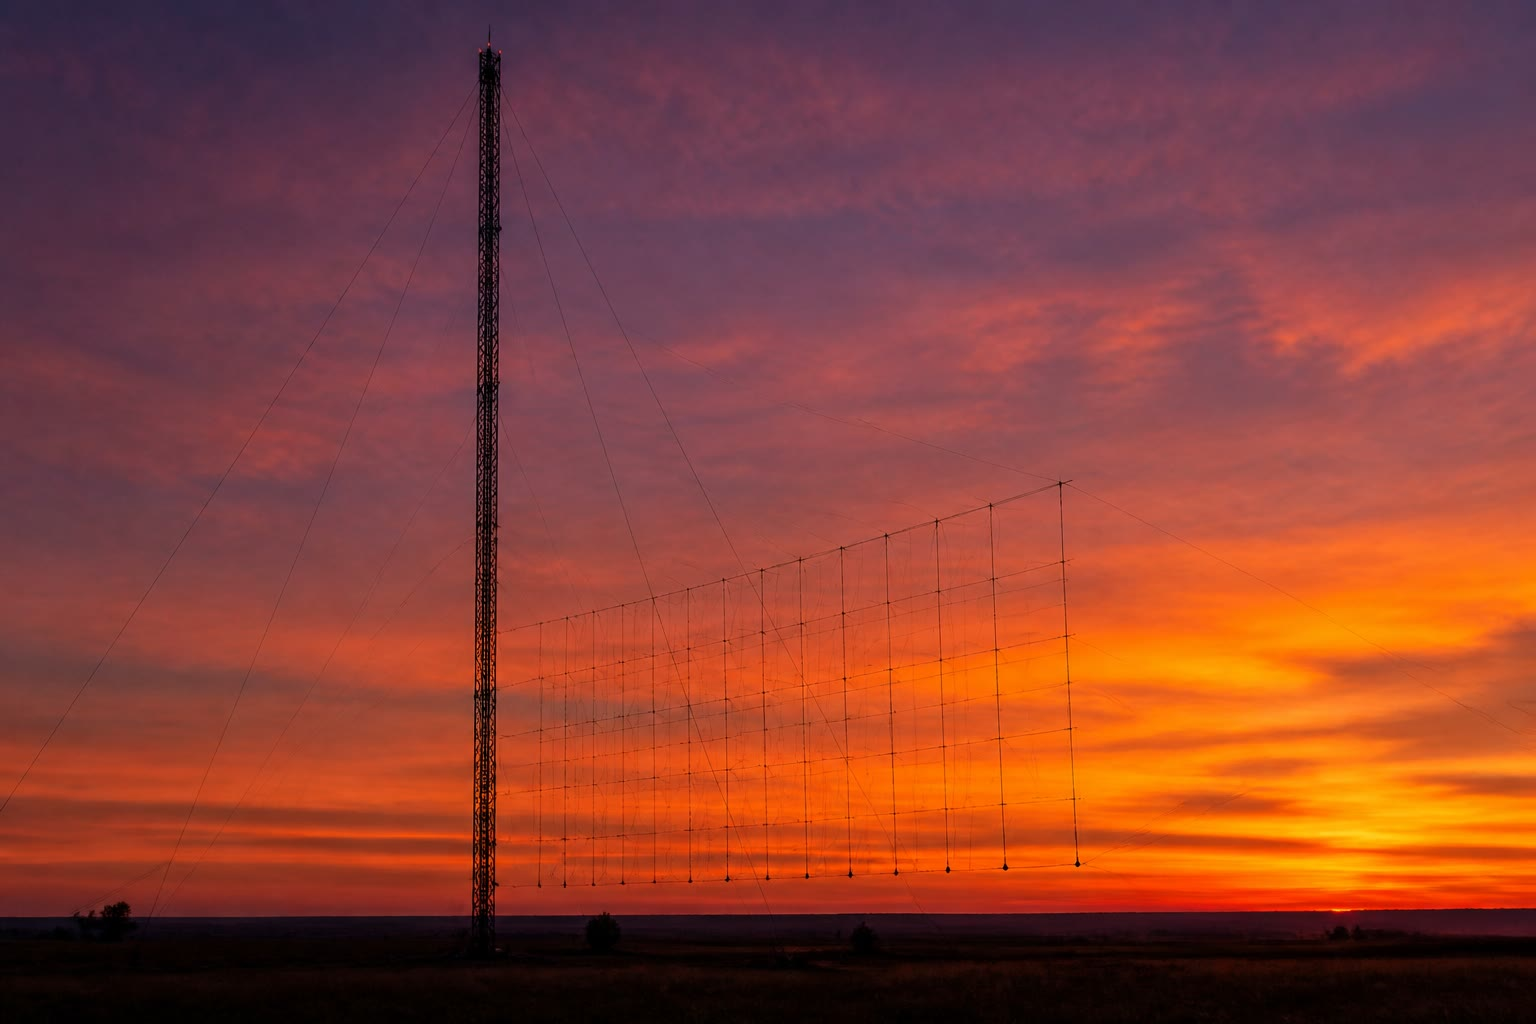
\includegraphics[width=0.58\linewidth]{images/book4/ai/b4-14-shortwave-antenna-sunset.jpg}

{\small 黄昏时的短波发射站：其波的频率比电离层等离子体频率低几兆赫，即将被反射回一千千米外的地面。}
\end{omfigure}

\begin{omfigure}
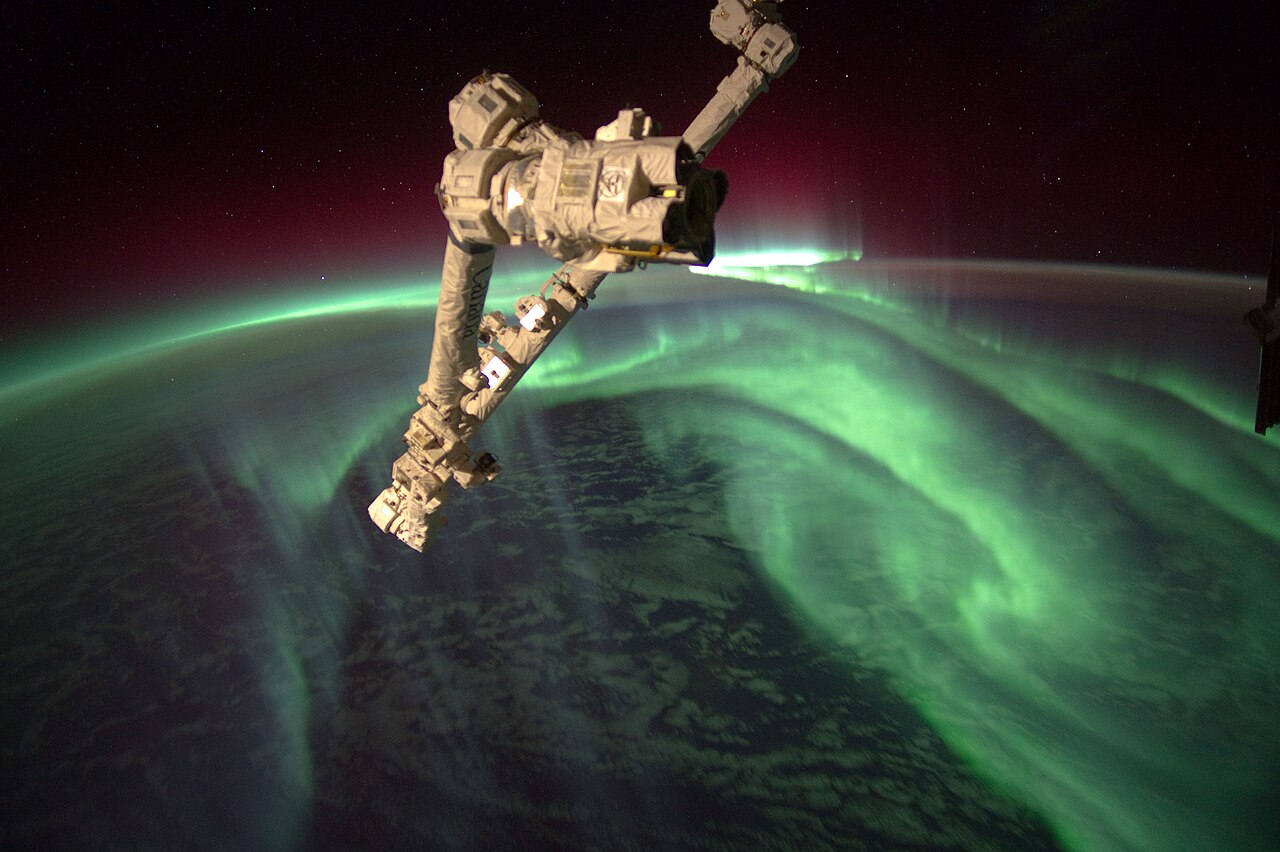
\includegraphics[width=0.6\linewidth]{images/book4/aurora-australis-iss.jpg}

{\small 从国际空间站拍摄的南极光：来自太阳的粒子受地球磁场引导，激发高层大气的等离子体——即其等离子体频率能反射无线电波的电离层（NASA）。}
\end{omfigure}

\section{问题：电离层、微波炉门与棱镜}

\begin{problem}[{周末问题——波所“看见”的三种材料：使
GPS 信号弯曲的等离子体、把微波留住的金属，以及
使白光色散的玻璃}]
\label{pb:b2:waves-in-media:1}

\medskip
\noindent\textbf{第一部分——电离层与 GPS。}
F 层的电子密度 $n = \qty{1e12}{m^{-3}}$；白天沿竖直路径的电子总柱
密度为 $N_T = \int n\,\dd z = \qty{2e17}{m^{-2}}$。
GPS：$f_1 = \qty{1575}{MHz}$，$f_2 = \qty{1228}{MHz}$。
\begin{enumerate}
  \item 求 F 层的等离子体频率；GPS 信号能否穿过？
        \qty{5}{MHz} 的短波能否穿过？
  \item 证明当 $\omega \gg \omega_p$ 时，群速度为 $v_g \approx c(1 -
        \omega_p^2/2\omega^2)$，相速度为 $c(1 + \omega_p^2/2\omega^2)$。
  \item GPS 信号穿过该层时的额外群延迟：证明
        $\Delta t = \dfrac{e^2}{8\pi^2\varepsilon_0mc}\,\dfrac{N_T}{f^2}$，并对
        $f_1$ 计算该值；求测距误差 $c\,\Delta t$。
  \item 接收机同时使用两个频率：由两个延迟可
        消去该误差。将 $N_T$ 用 $\Delta t_1 - \Delta t_2$ 表示；
        延迟之差需要达到多高的精度，才能使 $N_T$ 的误差为 $1\%$？
  \item 第 3 题中的延迟在
        $f_1$ 处相当于多少个额外的载波周期？
  \item 载波相位被\emph{提前}的量恰与
        群延迟的量相同：为何（两种修正的符号）？
        哪一项对于计数
        载波周期的接收机更重要？
  \item 夜间 $N_T$ 降至十分之一：单频接收机在
        白天与夜间的误差各为多少？
  \item 太阳耀斑使 D 层（\qty{80}{km}）的 $n$ 升至
        \qty{1e10}{m^{-3}}，且碰撞频繁：哪些无线电服务
        会受影响，为何 GPS 只受轻微影响？
\end{enumerate}

\medskip
\noindent\textbf{第二部分——烤箱门。}
腔壁与门网均为钢质（$\gamma = \qty{1.0e6}{S/m}$）；
门网孔宽 \qty{1.0}{mm}，网板厚 \qty{0.5}{mm}；
频率 $f = \qty{2.45}{GHz}$，功率 $P = \qty{800}{W}$。
\begin{enumerate}[resume]
  \item 求钢在 \qty{2.45}{GHz} 下的趋肤深度；壁是否“厚”？
  \item 表面电阻 $R_s = 1/\gamma\delta$；壁面表面磁场幅值
        为 $H_0 = \qty{30}{A/m}$（壁面面积 \qty{1}{m^2}）的情形下，
        壁中单位面积损耗功率为 $\tfrac12R_sH_0^2$，求其占
        $P$ 的比例。
  \item 在宽度 $a \ll \lambda$ 的孔中，场不能传播（该孔相当于
        截止以下的波导，见\cref{ch:b2:guided-waves}）：
        场按 $\eu^{-\pi z/a}$ 沿厚度 $z$ 衰减，
        求穿过 \qty{0.5}{mm} 网板时幅值的衰减量（以 dB 计）。
  \item 为何能透过网孔看到外面（将光的波长与孔径相比），
        而微波却无法穿出？
  \item 玻璃窗为电介质，其 $\underline\varepsilon_r = 4 - 0.02\iu$：
        求其折射率及其中光强的衰减长度；
        玻璃是否会被加热？
  \item 烤箱中有一把金属叉，其尖端处的场被增强；
        利用第 8 题的趋肤深度，估算
        表面电流密度（取 $H_0 = \qty{300}{A/m}$，表面处取 $j \approx H_0/\delta$），
        以及局部发热 $j^2/\gamma$——为何会产生火花？
\end{enumerate}

\medskip
\noindent\textbf{第三部分——射频下的导线。}
一根半径 $a = \qty{0.5}{mm}$（$\gamma = \qty{6e7}{S/m}$）的铜线，
位于 \qty{13.56}{MHz} 的感应加热线圈中，通有有效值为 \qty{20}{A} 的电流。
\begin{enumerate}[resume]
  \item 求趋肤深度与有效导电截面，以及每米
        交流电阻与直流电阻的对比。
  \item 每米线圈导线耗散的功率，以及导线
        在对流冷却 $h = \qty{20}{W/(m^2.K)}$ 下所能达到的温度。
  \item 线圈在钢质工件中感应出电流（$\gamma =
        \qty{1e6}{S/m}$，热态时 $\mu_r \approx 1$）：求该处趋肤深度；为何感应加热只加热表层，
        以及这一特性如何用于
        齿轮的淬火？
  \item 为降低线圈损耗，将导线换为内部通水的 \qty{3}{mm}
        铜管：求每米新电阻；
        管的内侧是否通有电流？
  \item 铜中趋肤深度等于导线半径时，频率为多少？
        低于此频率时，何种近似取代
        “粗导线”公式？
\end{enumerate}

\medskip
\noindent\textbf{第四部分——棱镜。}
某玻璃的 $n(\lambda) = 1.500 + \qty{5.0e3}{nm^2}/\lambda^2$，其共振
位于 $\lambda_0 = \qty{100}{nm}$。
\begin{enumerate}[resume]
  \item 验证柯西形式在远低于共振处可由洛伦兹模型导出，
        并验证 $\omega_p^2/\omega_0^2 = n^2(\infty) - 1$；求
        该玻璃的 $\omega_p^2/\omega_0^2$ 值及有效 $n$。
  \item 求 \qty{400}{nm} 与 \qty{700}{nm} 处的折射率与相速度，
        求 \qty{550}{nm} 处的群折射率；求两种颜色
        在此种玻璃光纤中传播 \qty{1}{km} 后的延迟。
  \item 顶角为 \qty{60}{\degree} 的棱镜，对 \qty{550}{nm} 光处于最小偏向时：
        求偏向角（用 $n\sin(A/2) = \sin((A + D)/2)$）；
        求 \qty{400}{nm} 与 \qty{700}{nm} 之间的角距离（求导）；在相距
        \qty{2}{m} 的屏幕上，光谱的宽度。
  \item 为何该玻璃在 \qty{200}{nm} 处不透明，
        若微量的铁使玻璃在 \qty{700}{nm} 处增加一个弱共振，其颜色如何？
  \item 在洛伦兹图像中，为何棱镜使蓝光
        比红光偏折得更厉害？
  \item 用一张表列出：对 F 层、钢、铜与玻璃，
        在各自工作频率下
        $\underline\gamma$ 的性质及波的去向。
\end{enumerate}
\end{problem}
